\documentclass{article}
\usepackage[preprint]{caisc_2026}
\usepackage[utf8]{inputenc}
\usepackage[T1]{fontenc}
\usepackage{hyperref}
\usepackage{url}
\usepackage{booktabs}
\usepackage{amsfonts}
\usepackage{amsmath}
\usepackage{nicefrac}
\usepackage{microtype}
\usepackage{xcolor}
\usepackage{graphicx}
\usepackage{subcaption}

\title{When Collapse Censors Drift: Differential Encoder Collapse Pre-empts Regularizer--Protocol Attribution in Latent World Models}

\author{%
  Anonymous Author(s)\\
  Affiliation\\
  Address\\
  \texttt{email}
}

\begin{document}

\maketitle

\begin{abstract}
Rollout drift, the compounding of prediction error during multi-step latent imagination, limits the use of world models for long-horizon planning. A prior controlled study attributed drift primarily to the training protocol (1-step teacher forcing versus multi-step closed-loop BPTT) rather than to the marginal regularizer, but implemented ``SIGReg'' as a moment-matching proxy. We pre-registered a follow-up with a faithful sliced Epps--Pulley statistic: a 3-regularizer $\times$ 2-protocol $\times$ 5-environment factorial (201 runs) with ground-truth-normalized metrics, collapse-as-outcome analysis, and an interventional encoder-swap probe. The pre-registered attribution contrasts were largely \emph{censored by differential collapse}: every unregularized run collapsed, and the Epps--Pulley regularizer, at weights selected by standard validation prediction error, produced dimensional or variance collapse on three of four non-bridge environments, while the crude moment proxy survived almost everywhere. We identify a candidate mechanism: exact collapse is a stationary point of the Epps--Pulley loss whose value ($1+\nicefrac{1}{\sqrt3}-\sqrt2\approx0.163$ at $\gamma{=}\nicefrac12$) matches the observed final loss of collapsed runs to four digits, and the statistic is bounded there, whereas the moment penalty grows as the latent dimension. On the one environment where both regularizers survived (Lorenz), closed-loop training reduced integrated rollout error in all five seeds under both regularizers (geometric ratios $0.046$ and $0.30$), with a short-horizon cost and long-horizon benefit, and regularizer differences were concentrated under 1-step training. We argue that collapse acts as a post-treatment intercurrent event, analogous to truncation by death, that can leave otherwise clean factorial drift studies unidentified, and must be reported as a primary outcome wherever marginal regularizers are compared.
\end{abstract}

\section{Introduction}
\label{sec:intro}

Latent world models compress observations $o_t$ into latents $z_t=\mathrm{enc}(o_t)$ and learn a transition $f$ with $z_{t+1}\approx f(z_t,a_t)$, then plan by rolling $f$ forward in imagination \citep{hafner2023dreamerv3,lecun2022path}. When rollouts drift, imagined futures diverge from reachable ones, and planners that optimize over imagined trajectories inherit the error \citep{zhou2024dinowm,sobal2025planning}. Two accounts of drift circulate. One blames the marginal regularizer: objectives such as SIGReg \citep{balestriero2025lejepa} constrain the aggregate distribution $q(z)$ but not the conditional $p(z_{t+1}\mid z_t)$, so fixing the regularizer is held to be the path to stable rollouts. The other blames the training protocol: models supervised only on one-step transitions from encoded states are never trained on their own predictions, a mismatch long known in sequence modeling \citep{lamb2016professor}, and multi-step closed-loop training is the corrective.

A prior controlled study \citep{anon2026drift} concluded that the protocol dominates: 1-step teacher forcing produced exploding perturbation amplification even on a contractive linear system, and 5-step BPTT largely repaired it. That study, however, implemented ``SIGReg'' as the moment proxy $\lVert\mu\rVert^2+\lVert\Sigma-I\rVert_F^2$. Since the distinctive content of SIGReg is its characteristic-function test of full normality, the most serious objection to the prior result is that its regularizer arm never contained the regularizer under discussion.

This paper is the pre-registered follow-up. We fixed the regularizer arm (a sliced exact-integral Epps--Pulley statistic, Section~\ref{sec:regularizers}), added environments spanning stationary-Gaussian, chaotic, action-conditioned, and pixel-observed regimes, normalized drift by ground-truth amplification, pre-registered contrasts and decision criteria, and added an interventional encoder-swap probe. We committed in advance to publishing whichever verdict the data supported: regularizer, protocol, interaction, mechanism, environment dependence, or null.

The data returned a verdict we had not enumerated: the pre-registered attribution contrasts were largely \emph{censored by differential collapse}. Every unregularized run collapsed (50/50). The Epps--Pulley regularizer, at weights selected by validation prediction error, collapsed on three of four non-bridge environments (33/33 main-factorial runs there), while the moment proxy survived almost everywhere. The comparison the field wants, faithful SIGReg versus nothing on drift, does not exist in this regime because ``nothing'' does not survive, and at the selected weights the faithful statistic often does not either.

We make three claims, scoped to this finite-training, overcomplete-latent regime. \textbf{(C1)} Regularizer choice acted primarily as a representation-viability gate: differential collapse pre-empted the pre-registered regularizer-versus-none drift contrasts in most environments, and the failure was invisible to one-step validation error. Its direct effect on drift therefore remains unidentified here, not refuted. \textbf{(C2)} Where both regularized conditions survived (Lorenz), closed-loop training reduced integrated rollout error in every seed under both regularizers, trading a short-horizon penalty for a large long-horizon gain, and regularizer differences appeared only under 1-step training (an exploratory interaction pattern). \textbf{(C3)} Mechanistically, exact collapse is a stationary point of the Epps--Pulley loss with a small bounded value that matches the observed final losses of collapsed runs to four digits, whereas the moment penalty at collapse grows with latent dimension; bounded saturation of the anti-collapse penalty is a candidate explanation for why the faithful statistic is the more collapse-prone one.

\section{Related Work}
\label{sec:related}

\textbf{JEPA world models and SIGReg.} LeJEPA \citep{balestriero2025lejepa} motivates an isotropic Gaussian embedding target and introduces SIGReg, which tests random one-dimensional projections for normality with an Epps--Pulley statistic. LeWorldModel \citep{maes2026lewm} trains an end-to-end JEPA world model from pixels with next-embedding prediction plus SIGReg and no stop-gradients, EMA encoders, or reconstruction; our minimal recipe mirrors it at small scale. KerJEPA \citep{zimmermann2025kerjepa} identifies the Epps--Pulley regularizer as a sliced Gaussian-kernel MMD, licensing the closed-form variant we use. Fast LeWorldModel \citep{gao2026fastlewm} attributes accumulated latent error to autoregressive one-step rollout and changes the inference interface; we exclude interface changes to keep the protocol factor clean.

\textbf{Exposure bias.} The teacher-forcing/free-running mismatch is classical \citep{lamb2016professor}; recent work frames recursive forecasting failure as epistemic underidentification \citep{green2026exposure}. Our protocol factor operationalizes this axis in latent space.

\textbf{Collapse in self-supervised learning.} Collapse avoidance is central to non-contrastive SSL, and LeJEPA positions SIGReg as the principled device. Our results support the anti-collapse framing with a twist: the collapse behavior of the faithful statistic is strongly environment- and weight-dependent in the world-model setting, and its failure mode is quiet.

\textbf{Censoring by intercurrent events.} Conditioning on a post-treatment variable biases causal contrasts; in clinical trials, death before outcome measurement (``truncation by death'') is the canonical case. We import this lens: collapse is an intercurrent event for drift measurement.

\section{Experimental Design}
\label{sec:design}

The design was written and externally reviewed before any GPU run; all deviations are in the ledger of Appendix~\ref{app:deviations}. Code, manifests, and analysis are in the supplement.

\subsection{Model and Training Protocols}
\label{sec:protocols}

All conditions share one architecture: an encoder (2-layer MLP, width 128, $d{=}16$ for state observations; 4-block CNN, $d{=}32$ for pixels) and a transition MLP over $[z,a]$. No decoder, reward head, stop-gradient, or EMA target: prediction plus regularization are the only losses, matching the minimal LeWorldModel recipe.

\textbf{P0 (1-step teacher forcing):} $\mathcal{L}_{\text{pred}}=\lVert f(\mathrm{enc}(o_t),a_t)-\mathrm{enc}(o_{t+1})\rVert_2^2$.
\textbf{P1 ($H$-step closed-loop BPTT), $H{=}8$:} $\hat z_{t+k}=f(\hat z_{t+k-1},a_{t+k-1})$ from $\hat z_t=\mathrm{enc}(o_t)$, $\mathcal{L}_{\text{pred}}=\frac1H\sum_{k}\lVert \hat z_{t+k}-\mathrm{enc}(o_{t+k})\rVert_2^2$.
\textbf{P0.5 ($H$-step teacher forcing, control):} dense multi-horizon targets, each step conditioned on the encoded previous observation; run on a subset to separate supervision density from closed-loop exposure.

\subsection{Regularizers}
\label{sec:regularizers}

\textbf{R0 (none):} $\mathcal{L}=\mathcal{L}_{\text{pred}}$.
\textbf{R1 (moment proxy, bridge):} $\mathcal{L}_{\text{reg}}=\lVert\mu_B\rVert_2^2+\lVert\Sigma_B-I\rVert_F^2$, reproducing the prior study's condition.
\textbf{R2 (sliced exact-integral Epps--Pulley):} for latents $Z\in\mathbb{R}^{B\times d}$ at one time point and $M{=}256$ random unit directions $u_m$, with $h=Zu_m$ and $\gamma{=}\nicefrac12$,
\begin{equation}
\label{eq:ep}
\mathrm{EP}_\gamma(h)=\tfrac{1}{B^2}\textstyle\sum_{i,j}e^{-\gamma(h_i-h_j)^2}+\tfrac{1}{\sqrt{1+4\gamma}}-\tfrac{2}{B\sqrt{1+2\gamma}}\textstyle\sum_i e^{-\gamma h_i^2/(1+2\gamma)},
\end{equation}
and $\mathrm{SIGReg}(Z)=\frac1M\sum_m \mathrm{EP}_\gamma(Zu_m)$. Equation~\eqref{eq:ep} is the exact integral of the Epps--Pulley characteristic-function statistic under a Gaussian weighting, equivalently a sliced Gaussian-kernel MMD to $\mathcal{N}(0,1)$ \citep{zimmermann2025kerjepa}. It is a faithful full-distribution normality test, unlike R1, but it is not numerically identical to the official quadrature estimator of \citet{balestriero2025lejepa}; all claims are implementation-specific and we write ``EP-SIGReg'' below.

Regularizer exposure is equalized across protocols: the statistic is computed per time point on the full batch and averaged over the time points visible to that protocol's loss, never on a flattened pool of temporally correlated frames. Under the main design R1/R2 apply only to encoded latents, never to rolled-out predictions.

\textbf{Weight selection.} $\lambda$ was tuned per (regularizer, environment) on $\{0.01,0.03,0.1,0.3,1.0\}$, seed 0, by validation one-step MSE \emph{subject to non-collapse diagnostics}, never on rollout metrics, and frozen across protocols, so tuning cannot manufacture a regularizer--protocol interaction. When every grid point failed the collapse screen, the selector fell back to best validation MSE; this fallback and its consequences are audited in Section~\ref{sec:collapse-results} and Appendix~\ref{app:lambda}.

\subsection{Environments}
\label{sec:envs}

\textbf{E0-det (bridge only):} deterministic stable linear, $x_{t+1}=Ax_t$, eigenvalues $\{0.7,0.8,0.9\}$; the prior study's sanity check, retained for R0/R1 bridge cells.
\textbf{E0 (stationary OU):} same contraction with noise calibrated so the marginal is $\mathcal{N}(0,I_3)$ at every step; SIGReg's favorable regime by construction, added because a time-varying marginal makes the Gaussian target unfair to it.
\textbf{E1 (Lorenz):} $\sigma{=}10,\rho{=}28,\beta{=}\nicefrac83$, $dt{=}0.01$; chaotic, so drift must be measured as excess over ground truth.
\textbf{E2/E3 (action-conditioned point mass, state/pixels):} identical clipped dynamics; E3 renders $64{\times}64$ grayscale frames, isolating the pixel-encoder axis.

\subsection{Metrics, Collapse Rule, and Pre-Registered Criteria}
\label{sec:metrics}

The primary outcome is \textbf{integrated probe-space open-loop error}: a ridge probe from $z$ to true state is fit on training data; the model rolls out freely along held-out action sequences; probe-space error against the true trajectory is integrated over horizons $1..50$. Probe space makes different latent geometries commensurable, and error against the \emph{true} trajectory means over-contraction scores badly, unlike signed amplification ratios that reward collapsed sensitivity. Amplification fidelity $|\log(A_{\text{model},25}/A_{\text{gt},25})|$ is secondary.

\textbf{Collapse rule.} A run is flagged when effective latent dimension $<2$, rank$_{1\%}<2$, or probe $R^2<0.5$ on state-recoverable environments. Because these axes differ, we decompose flagged runs into \emph{variance} collapse (near-zero scale), \emph{dimensional} collapse (rank-deficient but decodable), and \emph{informational} collapse (probe failure) in Section~\ref{sec:collapse-results}. Collapse is an outcome; drift conditional on survival is reported with the conditioning explicitly treated as post-treatment selection.

\textbf{Pre-registered contrasts.} On the log primary outcome with seeds as paired blocks and cluster bootstrap over seeds: $C_R=(\text{R2}-\text{R0})$ under P0; $C_P=(\text{P1}-\text{P0})$ averaged over R0 and R2; $C_I$ the protocol difference of $C_R$; equivalence margin $\log 1.25$. Verdict definitions preceded execution (Appendix~\ref{app:prereg}). We supplement the bootstrap with exact paired sign-flip tests and leave-one-seed-out estimates, since $n{=}5$ seeds bound what a bootstrap can certify.

\textbf{Encoder-swap probe.} On E0, encoders from P0- and P1-trained R2 runs (seeds 0--2) are frozen and dynamics retrained under both protocols, a full $2{\times}2$ with retrained diagonals.

\textbf{Scale.} 45 $\lambda$-pilot runs, 144 factorial/control runs, 12 swap runs on $7{\times}$ NVIDIA L4, under \$20 total. Mid-execution, a wall-clock constraint forced a uniform training-step reduction (state $20\text{k}{\to}10\text{k}$, visual $15\text{k}{\to}8\text{k}$) and the dropping of the $\lambda$-sensitivity, matched-dimension, and $M{=}1024$ arms; the deviation ledger is Appendix~\ref{app:deviations}.

\section{Results}
\label{sec:results}

\subsection{Differential Collapse Censors the Pre-Registered Contrasts}
\label{sec:collapse-results}

\begin{figure}[t]
  \centering
  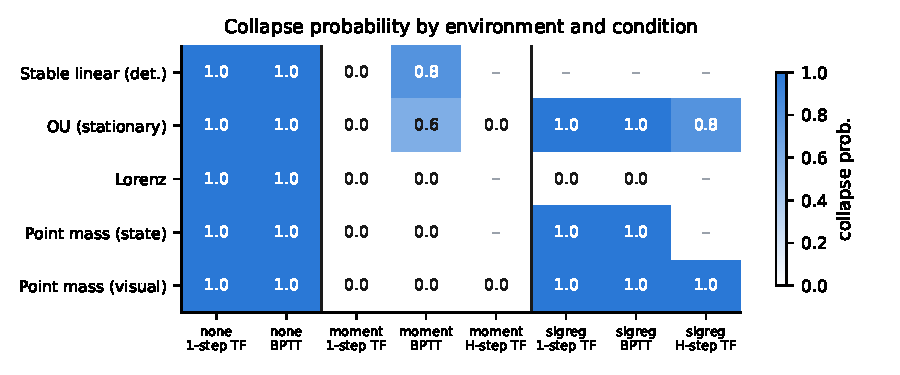
\includegraphics[width=0.9\linewidth]{figures/fig1_collapse_matrix.pdf}
  \caption{Collapse probability by environment and condition (seeds pooled; ``--'' = not in design). Every unregularized run collapsed. EP-SIGReg at validation-selected $\lambda$ collapsed on OU and both point-mass environments under every protocol, surviving only on Lorenz. The moment proxy is the most collapse-robust condition.}
  \label{fig:collapse}
\end{figure}

Figure~\ref{fig:collapse} shows the result that reorganizes the paper. \textbf{R0 collapsed in 50/50 runs}: with prediction loss alone this minimal recipe has no surviving optimum in any environment, under either protocol. \textbf{R2 collapsed in 33/33 main-factorial runs on OU and both point-mass environments} (and 4/5 under P0.5 on OU) while surviving 10/10 on Lorenz. \textbf{R1 survived} everywhere under P0 and in most other cells (60\% collapse OU/P1; 80\% E0-det/P1).

Decomposing the flag: of 33 collapsed R2 runs, 19 are \emph{variance} collapse (near-zero scale), 5 \emph{dimensional} (rank $<2$ yet probe $R^2$ 0.67--0.79 on OU: state still decodable on a degenerate manifold), 9 \emph{informational} (probe failure, mostly point-mass). ``Collapse'' here therefore does not always mean information loss, and we use the criterion-specific term throughout.

\textbf{The $\lambda$ audit.} The selection protocol chose $\lambda{=}1.0$ (the grid boundary) for R2 on OU and Lorenz; on both point-mass environments \emph{every} R2 grid point failed the pilot collapse screen, so the fallback selected by validation MSE alone, which under collapse favors the most degenerate solution (validation one-step MSE of a collapsed code is spuriously tiny: $4{\times}10^{-7}$ on OU). The honest statement is not ``EP-SIGReg collapses world models'' but: \emph{at weights chosen by a standard validation protocol, the faithful statistic produced degenerate latents on three of four environments, and the failure is invisible, indeed attractive, to one-step validation error}. Whether other weights avoid this is unresolved here (the $\lambda$-sensitivity arm was dropped; Section~\ref{sec:limits}).

\textbf{A candidate mechanism.} At exact collapse ($Z\equiv0$), every projection is degenerate and Eq.~\eqref{eq:ep} evaluates to $1+\nicefrac{1}{\sqrt3}-\sqrt2\approx0.1631$ at $\gamma{=}\nicefrac12$: a stationary point of the regularizer with a small, \emph{bounded} value (the statistic is an MMD, bounded by construction). The observed final regularizer loss of the 33 collapsed R2 runs has median exactly $0.1631$ (range $0.103$--$0.163$). The moment penalty at the same point is $\lVert -I\rVert_F^2=d=16$: unbounded in dimension and two orders of magnitude larger. Once trajectories approach the collapsed stationary point, the EP penalty offers a vanishing restoring force while the moment penalty does not. We present this as a candidate optimization-level explanation consistent with the losses we log, not as a proven cause; it yields a directly testable prediction (collapse frequency should fall with penalties that diverge at degeneracy, or with warm starts away from the stationary point).

\subsection{Where Both Regularizers Survive: Protocol Effects and an Exploratory Interaction}
\label{sec:lorenz}

\begin{figure}[t]
  \centering
  \begin{subfigure}{0.44\linewidth}
    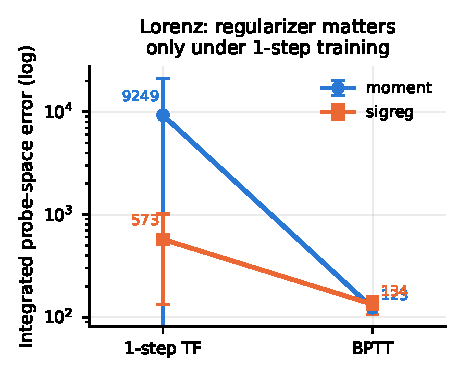
\includegraphics[width=\linewidth]{figures/fig2_lorenz_interaction.pdf}
  \end{subfigure}\hfill
  \begin{subfigure}{0.50\linewidth}
    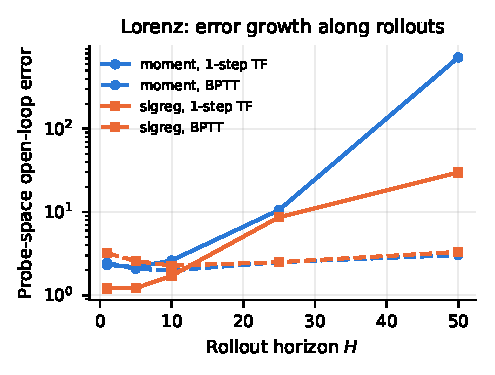
\includegraphics[width=\linewidth]{figures/fig3_lorenz_horizons.pdf}
  \end{subfigure}
  \caption{Lorenz, the only environment where R1 and R2 both survive both protocols. Left: integrated probe-space rollout error (mean $\pm$ 95\% CI over 5 seeds, log scale). Right: error growth by horizon; closed-loop training is \emph{worse} at $H{=}1$ and much better at $H{=}50$.}
  \label{fig:lorenz}
\end{figure}

Lorenz is the single environment where R1 and R2 are both fully evaluable ($C_R$ against R0 remains censored even here, since R0 collapsed). Because the pre-registered $C_P$ averages over R0, it too is formally unevaluable; we therefore report $C_{P\mid R2}$ and $C_{P\mid R1}$ and label them as such. Moving P0${\to}$P1 reduced the log primary outcome in \emph{all five seeds under both regularizers}: geometric ratios $0.046$ under R1 (mean log effect $-3.09$, seed-blocked bootstrap CI $[-4.6,-1.7]$) and $0.30$ under R2 ($-1.20$, CI $[-1.75,-0.65]$); exact two-sided sign-flip $p=0.0625$ for each, the minimum attainable with five seeds, with leave-one-seed-out ranges $[-3.7,-2.4]$ and $[-1.4,-1.0]$.

The horizon profile (Figure~\ref{fig:lorenz}, right) shows this is a genuine tradeoff, not uniform improvement: under R2, closed-loop training is $2.6\times$ \emph{worse} at $H{=}1$ and $0.16\times$ at $H{=}50$ (under R1: $1.06\times$ and $0.018\times$). Closed-loop training buys long-horizon stability at short-horizon cost, consistent with exposure to self-generated states rather than better one-step modeling.

The regularizer comparison is exploratory (it was not a pre-registered contrast): under P0, R2 beats R1 by a geometric factor of $6.2$ (mean log difference $-1.82$; sign-flip $p=0.125$); under P1 the two are indistinguishable (ratio $1.07$, $p=0.56$). The interaction pattern, regularizer choice mattering only under the deficient protocol, is thus descriptive with $n{=}5$: visible in the means, not certified by the exact test ($p=0.19$).

\begin{figure}[t]
  \centering
  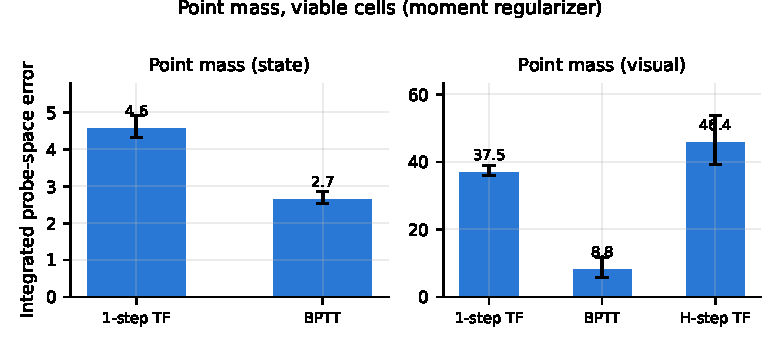
\includegraphics[width=0.7\linewidth]{figures/fig4_pointmass_protocol.pdf}
  \caption{Point-mass environments, surviving cells (R1 only). Closed-loop training reduces integrated rollout error on both; the dense teacher-forcing control (P0.5) does not, isolating closed-loop exposure rather than supervision density as the operative ingredient.}
  \label{fig:pointmass}
\end{figure}

The point-mass environments corroborate the protocol direction where cells survive (R1 only): $4.6{\to}2.7$ (state) and $37.5{\to}8.8$ (visual) moving P0${\to}$P1, and the P0.5 dense-supervision control lands at $46.4$, no better than P0 (Figure~\ref{fig:pointmass}).

\subsection{The Encoder-Swap Probe Returns a Null}
\label{sec:swap}

All twelve swap runs on OU inherited the R2-on-OU dimensional-collapse regime, and the primary outcome was flat across the $2{\times}2$ ($\approx80\pm5$; OU's rollout-error noise floor is $\approx76$). The probe is uninformative in this regime: OU error saturates near the floor for degenerate and healthy models alike. We report a null of the probe, not of the mechanism.

\subsection{Verdict Against the Pre-Registered Criteria}
\label{sec:verdict}

$C_R$: \textbf{censored} (no surviving R0 cell anywhere). $C_P$ as pre-registered (averaged over R0, R2): \textbf{censored}; the conditional versions $C_{P\mid R1},C_{P\mid R2}$ are supported on Lorenz with all-seed consistency, and directionally corroborated on point-mass under R1. $C_I$: censored; the descriptive interaction on Lorenz does not reach exact-test significance. Encoder-geometry: probe null under collapse. Formal verdict: \textbf{mixed}, and the substantive content of the paper is C1--C3 of Section~\ref{sec:intro}. We emphasize what this verdict is not: it is not ``protocol dominates'' as pre-registered (that criterion required two dynamics families and $C_R$ equivalence), and it is not ``SIGReg fails'' (the weight-selection audit blocks that reading).

The bridge to the prior study also degraded: on E0-det, R1/P1 flagged 4/5 seeds while R1/P0 survived cleanly, so the prior paper's cleanest environment did not reproduce under our shorter training budget. Training length, $\lambda$, metric, and implementation all changed; we flag the non-reproduction rather than adjudicate it.

\section{Limitations}
\label{sec:limits}

(1) \textbf{Weight selection is the largest confound}: the $\lambda$-sensitivity arm was dropped under the wall-clock constraint, R2's selected weights sat at the grid boundary or arose from an all-collapsed fallback, and R1/R2 loss scales differ so the shared numerical grid is not dose-matched. All collapse claims are ``at the selected weights.'' (2) The uniform step reduction is condition-uniform but not treatment-neutral: conditions may converge or collapse at different rates, so claims hold at the observed training horizon; the bridge non-reproduction makes this concrete. (3) R2 is an exact-integral EP variant; the pre-registered parity test against the official quadrature implementation was not executed. (4) Three pre-registration violations discovered in post-hoc code audit: final metrics were computed on the validation split rather than the held-out test split; evaluation windows were sampled per run rather than from a fixed shared suite, weakening seed-pairing; and the regularizer's random projections consume the same RNG stream as minibatch sampling, so R2 conditions saw different minibatch sequences than R0/R1 at the same seed. (5) Environments are small and synthetic; the visual task is a single Gaussian-blob point mass; five (three visual) seeds per cell. (6) The matched-latent-dimension and $M{=}1024$ arms were dropped, leaving the overcomplete-latent explanation for R2's behavior untested.

\section{Conclusion}
\label{sec:conclusion}

We set out to test whether a faithful SIGReg overturns the protocol attribution of rollout drift, and mostly could not run the intended comparison: differential collapse censored it. What survives is, first, a conditional replication, where models live, closed-loop training reduces long-horizon rollout error in every seed, at short-horizon cost, and dense supervision without closed-loop exposure does not; second, an audited failure mode, a faithful normality statistic paired with standard validation-based weight selection can quietly select degenerate representations, plausibly because its penalty saturates at a bounded stationary point where cruder unbounded penalties do not; and third, a methodological rule we think generalizes: collapse is an intercurrent event for drift measurement, conditioning on survival is post-treatment selection, and factorial studies of world-model regularizers should pre-register collapse as a primary outcome and power their designs to remain identified when arms die.

\begin{ack}
Experiments, analysis, and writing were assisted by Claude (Anthropic), with human direction of the research question, compute budget, and final approval; external automated review at design and results stages was provided by OpenAI Codex. The full division of labor, including exact prompts, is documented in Appendix~\ref{app:session}. Compute: one RunPod $7{\times}$L4 instance, under \$20 of a \$30 budget.
\end{ack}

\bibliographystyle{plainnat}
\bibliography{references}

\newpage
\appendix

\section{Pre-Registered Decision Criteria (Verbatim Summary)}
\label{app:prereg}

The following criteria were fixed in \texttt{experiment\_design.md} before any paid GPU run, after two rounds of external automated review (one at design v1, one at v2/v3). Let $m=\log 1.25$ on the log primary outcome.

\begin{itemize}
\item \textbf{Regularizer fixes drift:} $C_R$ CI excludes 0 in the improving direction on $\geq 2$ of 3 dynamics families (the two point-mass environments count as one family), and the P0+R2 vs.\ P1 contrast CI lies entirely inside $[-m,m]$ (TOST-style equivalence), without collapse.
\item \textbf{Protocol dominates:} $C_P$ CI excludes 0 in $\geq 2$ of 3 families AND $C_R$ equivalence-to-zero holds.
\item \textbf{Interaction:} $C_I$ CI excludes 0 in $\geq 2$ families, or a CI-supported sign flip of $C_R$ between protocols.
\item \textbf{Encoder geometry:} in the swap $2{\times}2$, the primary outcome follows encoder source rather than dynamics-retraining protocol (interaction-contrast CI).
\item \textbf{Null/equivalence:} $C_R$, $C_P$, $C_I$ CIs all inside $[-m,m]$.
\item \textbf{Mixed:} anything else, reported as such with all contrast CIs.
\end{itemize}

Outcome: $C_R$, $C_P$, and $C_I$ were censored by differential collapse (no surviving R0 cell exists anywhere in the design); the realized verdict is \textbf{mixed}, with the conditional protocol contrasts $C_{P\mid R1}$, $C_{P\mid R2}$ supported on Lorenz. The collapse rule and the collapse-as-outcome analysis were themselves pre-registered, which is why the censoring is reportable rather than fatal.

\section{Deviation Ledger}
\label{app:deviations}

All deviations from the pre-registered design, with causes. Items 1--5 were forced by an 8-hour wall-clock constraint imposed mid-execution; items 6--8 were discovered in post-hoc code audit.

\begin{enumerate}
\item \textbf{Training steps reduced uniformly}: state $20\text{k}\!\to\!10\text{k}$, visual $15\text{k}\!\to\!8\text{k}$, identically for every condition. Uniform in treatment but not necessarily treatment-neutral (conditions may converge at different rates); all claims hold at the observed training horizon.
\item \textbf{Visual seeds} $5\to3$ (reverting to the original scope).
\item \textbf{Dropped arms}: $\lambda$-sensitivity (24 runs), matched latent dimension (24), $M{=}1024$ projections (2), rollout-regularization ablation (12). The $\lambda$-sensitivity drop is the most consequential (Section~5, Limitation 1).
\item \textbf{Encoder-swap restructured}: phase-A source models were taken from checkpointed core-sweep cells rather than trained separately (saving 12 runs); the $2{\times}2$ retains retrained diagonals.
\item \textbf{$\lambda$-pilot steps} reduced to 8k/4k (state/visual); pilots rank candidates, and all candidates within a cell share the budget.
\item \textbf{Validation split used for final metrics} instead of the generated test split (pre-registration specified test).
\item \textbf{Evaluation windows sampled per run} rather than from a fixed shared evaluation suite, weakening seed-pairing across conditions.
\item \textbf{Shared RNG stream}: the regularizer's random projections consume the same generator as minibatch sampling, so R2 conditions saw different minibatch sequences than R0/R1 at equal seed.
\item \textbf{SIGReg parity test not executed}: the pre-registered loss/gradient parity check against the official LeWorldModel implementation was specified but not run before the sweep; R2 claims are implementation-specific (exact-integral EP variant).
\end{enumerate}

\section{Weight-Selection Audit}
\label{app:lambda}

\begin{figure}[h]
  \centering
  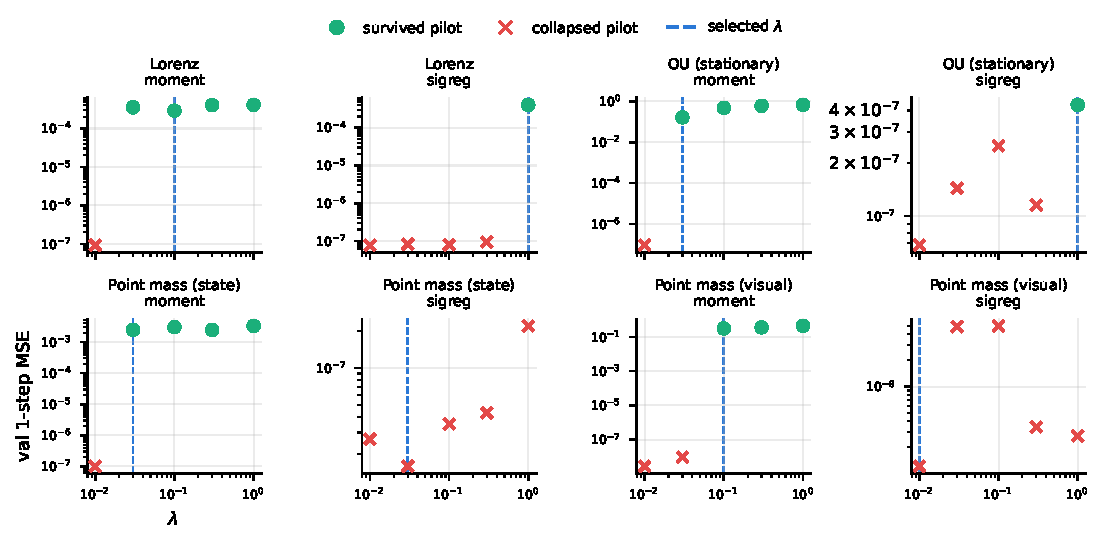
\includegraphics[width=\linewidth]{figures/fig7_lambda_frontier.pdf}
  \caption{The full $\lambda$-pilot grid (seed 0, 1-step protocol, reduced pilot budget): validation one-step MSE versus $\lambda$, colored by the pilot collapse screen. Collapsed pilots exhibit spuriously tiny validation MSE ($10^{-9}$--$10^{-7}$), which is why validation error alone cannot be trusted for weight selection. For EP-SIGReg on OU and Lorenz only the grid boundary $\lambda{=}1.0$ survived the screen; on both point-mass environments no grid point survived and the pre-registered fallback (best validation MSE among all candidates) then actively favored the most degenerate solution.}
  \label{fig:lambda}
\end{figure}

Table~\ref{tab:lambda} lists selections. Three structural observations: (i) at low $\lambda$ every regularizer collapses, as expected, since R0 always collapses; (ii) for EP-SIGReg the surviving region is empty (point mass) or a boundary point (OU, Lorenz); (iii) the OU boundary survivor at pilot length ($8$k steps, val MSE $4.3\times10^{-7}$, probe $R^2$ 0.89) slid into dimensional collapse at full length ($10$k steps) in 10/10 main runs, i.e.\ the pilot screen passed a configuration that was already en route to the collapsed stationary point.

\begin{table}[h]
\centering
\caption{Selected $\lambda$ per (regularizer, environment). ``All collapsed'' marks cells where no grid point passed the pilot collapse screen and the fallback selected on validation MSE alone.}
\label{tab:lambda}
\small
\begin{tabular}{llcc}
\toprule
Environment & Regularizer & Selected $\lambda$ & Pilot grid status \\
\midrule
Stable linear (det.) & moment & 0.01 & all 5 survived \\
OU & moment & 0.03 & 4/5 survived \\
OU & EP-SIGReg & 1.0 & only boundary survived \\
Lorenz & moment & 0.1 & 4/5 survived \\
Lorenz & EP-SIGReg & 1.0 & only boundary survived \\
Point mass (state) & moment & 0.03 & 4/5 survived \\
Point mass (state) & EP-SIGReg & 0.03 & \textbf{all collapsed} \\
Point mass (visual) & moment & 0.1 & 3/5 survived \\
Point mass (visual) & EP-SIGReg & 0.01 & \textbf{all collapsed} \\
\bottomrule
\end{tabular}
\end{table}

The R1 and R2 loss scales also differ substantially (the EP statistic is bounded; the moment penalty is not), so the shared numerical grid is not dose-matched between regularizers; between-regularizer collapse comparisons should be read with that in mind.

\section{The Collapsed Stationary Point of the Epps--Pulley Loss}
\label{app:stationary}

Let all latents be identical, $Z\equiv c$ for a constant $c\in\mathbb{R}^d$ (variance collapse; $c=0$ after any centering). Every projection is then the constant $h_i\equiv h_0=\langle c,u\rangle$. Substituting into Eq.~(1) of the main text:
\begin{align}
\mathrm{EP}_\gamma(h) &= \frac{1}{B^2}\sum_{i,j} e^{-\gamma(h_0-h_0)^2} + \frac{1}{\sqrt{1+4\gamma}} - \frac{2}{\sqrt{1+2\gamma}}\, e^{-\gamma h_0^2/(1+2\gamma)} \nonumber\\
&= 1 + \frac{1}{\sqrt{1+4\gamma}} - \frac{2}{\sqrt{1+2\gamma}}\, e^{-\gamma h_0^2/(1+2\gamma)}.
\end{align}
At $h_0=0$ and $\gamma=\nicefrac12$ this is $1+\nicefrac{1}{\sqrt3}-\sqrt2\approx 0.16308$. The sample--sample term is constant in $Z$ on the collapsed manifold and the sample--prior term is maximized at $h_0=0$, so $Z\equiv0$ is a stationary point of $\mathrm{EP}_\gamma$ (by symmetry of the Gaussian weighting, the gradient vanishes there), and because the statistic is an MMD it is \emph{bounded}: the penalty for total collapse saturates at $\approx0.163$ per projection. The empirical check: across the 33 collapsed EP-SIGReg runs in the main factorial, the median final regularizer loss is $0.1631$ (range $0.103$--$0.163$), matching the theoretical value to four digits, and 19/33 of those runs are variance collapses.

Contrast the moment proxy at the same point: $\lVert\mu\rVert^2+\lVert 0 - I\rVert_F^2 = \lVert c\rVert^2 + d$, which is at least $d=16$, two orders of magnitude larger, and grows with latent dimension. A trajectory approaching total collapse therefore feels a vanishing restoring force from the EP penalty but a large one from the moment penalty. We offer this as a candidate optimization-level explanation of the differential collapse pattern, consistent with the logged losses; establishing causality would require intervention (e.g., penalties modified to diverge at degeneracy, or warm starts displaced from the stationary point), which we leave to follow-up work.

Note the interplay with prediction: at $Z\equiv0$ the one-step prediction loss is also globally minimal (the dynamics maps $0\mapsto0$), so the collapsed configuration is a joint stationary point of the \emph{total} objective in which validation one-step MSE looks excellent. This is why the failure is invisible, indeed attractive, to validation-error-based model selection, and why the pilot screen's diagnostics (effective dimension, rank, probe $R^2$) are the only part of the selection protocol that resists it.

\section{Additional Results}
\label{app:extra}

\subsection{Collapse-Mode Decomposition}

Across all 144 factorial/control runs: 58 viable, 48 variance collapses, 8 dimensional, 30 informational. By regularizer (collapsed runs only): R0, 29 variance / 0 dimensional / 17 informational of 46; R1, 0/3/4 of 7; R2, 19/5/9 of 33. Figure~\ref{fig:effdim} shows the two collapse axes are genuinely distinct: a band of runs with effective dimension $<2$ retains probe $R^2>0.65$.

\begin{figure}[h]
  \centering
  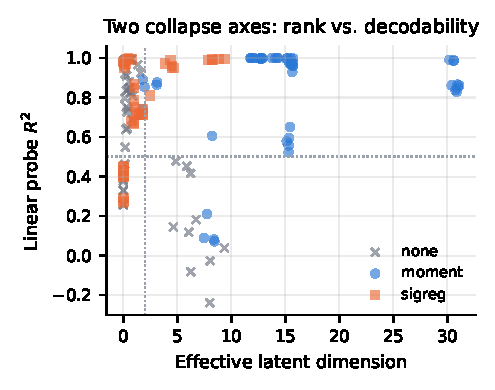
\includegraphics[width=0.55\linewidth]{figures/fig6_effdim_probe.pdf}
  \caption{Effective latent dimension versus linear-probe $R^2$, one point per run. Dotted lines mark the collapse thresholds. Rank-deficient codes (left of the vertical line) frequently remain decodable (above the horizontal line), which is why we report variance, dimensional, and informational collapse separately.}
  \label{fig:effdim}
\end{figure}

\subsection{Encoder-Swap $2{\times}2$}

\begin{figure}[h]
  \centering
  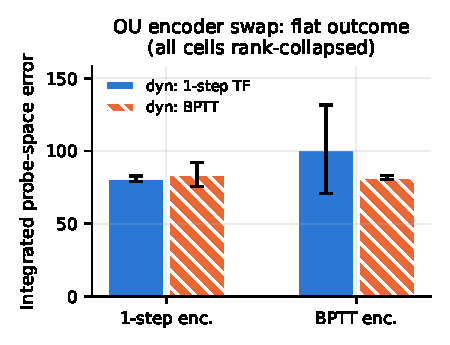
\includegraphics[width=0.5\linewidth]{figures/fig5_swap.pdf}
  \caption{Encoder-swap probe on OU (EP-SIGReg, seeds 0--2, retrained diagonals): integrated probe-space error is flat ($\approx80\pm5$) across all four encoder-source $\times$ dynamics-protocol cells; every cell is rank-collapsed and OU's rollout-error noise floor is $\approx76$. The probe is uninformative in this regime.}
  \label{fig:swap}
\end{figure}

\subsection{Lorenz Paired-Seed Detail}

Per-seed log effects of P1$-$P0 on the integrated primary outcome. Moment: $-1.84,-5.74,-2.70,-4.36,-0.80$ (mean $-3.09$; geometric ratio $0.046$; exact two-sided sign-flip $p=0.0625$; leave-one-out range $[-3.66,-2.42]$). EP-SIGReg: $-0.98,-2.17,-0.44,-0.70,-1.72$ (mean $-1.20$; ratio $0.30$; $p=0.0625$; LOO $[-1.39,-0.96]$). Exploratory regularizer contrast under P0 (R2$-$R1): mean $-1.82$ (ratio $0.162$, i.e.\ $6.2\times$ in R2's favor; $p=0.125$); under P1: $+0.06$ (ratio $1.07$; $p=0.56$). Horizon-resolved geometric ratios (P1/P0): moment $1.06,0.97,0.77,0.26,0.018$ and EP-SIGReg $2.63,2.08,1.29,0.34,0.16$ at $H=1,5,10,25,50$.

\subsection{Full Condition Summary}

\begin{table}[h]
\centering
\caption{All conditions: collapse probability and primary outcome conditional on survival (mean over surviving seeds; ``--'' = no survivors). Integrated probe-space open-loop error; lower is better; scales are environment-specific and not comparable across rows of different environments.}
\label{tab:full}
\small
\begin{tabular}{llccc}
\toprule
Environment & Reg. & Protocol & Collapse prob. & Primary $\mid$ viable \\
\midrule
Stable linear (det.) & none & P0 / P1 & 1.0 / 1.0 & -- / -- \\
Stable linear (det.) & moment & P0 / P1 & 0.0 / 0.8 & 2.99 / 2.68 \\
OU & none & P0 / P1 & 1.0 / 1.0 & -- / -- \\
OU & moment & P0 / P1 / P0.5 & 0.0 / 0.6 / 0.0 & 76.4 / 77.8 / 76.1 \\
OU & EP-SIGReg & P0 / P1 / P0.5 & 1.0 / 1.0 / 0.8 & -- / -- / 115.6 \\
Lorenz & none & P0 / P1 & 1.0 / 1.0 & -- / -- \\
Lorenz & moment & P0 / P1 & 0.0 / 0.0 & 9249 / 123 \\
Lorenz & EP-SIGReg & P0 / P1 & 0.0 / 0.0 & 573 / 134 \\
Point mass (state) & none & P0 / P1 & 1.0 / 1.0 & -- / -- \\
Point mass (state) & moment & P0 / P1 & 0.0 / 0.0 & 4.61 / 2.70 \\
Point mass (state) & EP-SIGReg & P0 / P1 & 1.0 / 1.0 & -- / -- \\
Point mass (visual) & none & P0 / P1 & 1.0 / 1.0 & -- / -- \\
Point mass (visual) & moment & P0 / P1 / P0.5 & 0.0 / 0.0 / 0.0 & 37.5 / 8.8 / 46.4 \\
Point mass (visual) & EP-SIGReg & P0 / P1 / P0.5 & 1.0 / 1.0 / 1.0 & -- / -- / -- \\
\bottomrule
\end{tabular}
\end{table}

\section{Compute Account}
\label{app:compute}

One RunPod instance, $7\times$ NVIDIA L4 24\,GB, 128 vCPUs. Total runs: 45 $\lambda$ pilots + 144 factorial/control + 12 swap = 201; zero failed jobs. A CPU-oversubscription pathology initially inflated per-step costs $\sim$$10\times$ (each PyTorch process spawned $\sim$35 threads; 7 concurrent jobs thrashed 128 vCPUs); capping \texttt{OMP\_NUM\_THREADS}=12 restored 96--98\% GPU utilization and roughly $3\times$ throughput. End-to-end wall clock from first pilot to finished analysis was under 3 hours against an 8-hour ceiling; total spend was under \$20 of a \$30 budget. Jobs were dispatched by a thread-safe GPU-pool runner (one job per GPU, round-robin) with stage-level hard-kill deadlines.

\section{Human--AI Session Flow and Division of Labor}
\label{app:session}

This study was conducted end-to-end by Claude (Anthropic; planning phases on Claude Fable 5, execution phases on Claude Sonnet 5) operating as an autonomous research agent under human direction, with OpenAI Codex (GPT-5-class, high reasoning effort) as an external automated reviewer at the design and results stages. The full machine-readable log is \texttt{session\_log.md} in the supplement. Summary of the division of labor:

\textbf{Human input.} (i) The research brief, verbatim: ``rollout drift in latent world models is caused by both the choice of marginal regularizer and the training protocol, and the two interact --- meaning neither can be studied in isolation [\dots] I don't want to specify what kinds of findings I'm looking for, because that would bias the experimental design. What I want from the results is honest engagement with the question --- experiments designed to distinguish between real possibilities rather than confirm a preferred answer.'' (ii) The compute budget (\$30 hard ceiling) and, mid-execution, an 8-hour wall-clock ceiling. (iii) Provisioning decisions: GPU vendor/type iterations (final: one $7\times$L4 instance) and SSH access. (iv) Approvals at phase boundaries; the instruction to proceed autonomously thereafter.

\textbf{AI work.} Literature positioning; adoption and revision of a prior interrupted session's design (v1) into v2--v4 under two external review rounds; all code (environments, regularizers, training protocols, metrics, sweep orchestration, GPU-pool runner, analysis); the $\lambda$ protocol; execution and monitoring on the remote instance; the mid-execution replan under the 8-hour constraint (uniform step reduction, arm drops, thread fix), logged before outcomes were seen; all statistical analysis including the post-review corrections (geometric effects, exact sign-flip tests, collapse-mode decomposition, stationary-point derivation and its empirical check); figures; and this manuscript.

\textbf{External automated review.} Codex review 1 (design stage) forced five major fixes before execution, including the stationary-Gaussian OU environment, the non-gameable primary metric, equalized regularizer exposure across protocols, contrast-based pre-registration with equivalence margins, and collapse-as-outcome analysis. Codex review 2 (results stage) corrected an arithmetic-mean effect size to its geometric value ($16\times\to6.2\times$), identified that the reported $C_P$ was actually $C_{P\mid R2}$, flagged the three pre-registration violations in the deviation ledger, proposed the collapse-mode decomposition and the $\lambda$-frontier audit, and contributed the observation that exact collapse is a stationary point of the EP loss with value $\approx0.163$, which we verified against the logged losses.

\textbf{Errors made and caught during the session} (retained for transparency): an initial GPU-dispatch bug that would have serialized all jobs onto one GPU (caught by utilization monitoring before damage); a stripped interpreter prefix that crashed all jobs instantly (caught within seconds); the CPU-thread oversubscription described in Appendix~\ref{app:compute} (caught by comparing isolated versus concurrent throughput); and an isolated-benchmark cost model that underestimated concurrent-load costs, corrected by re-benchmarking under realistic load before the main sweep.

\section{Reproducibility}
\label{app:repro}

The supplement contains: all source (\texttt{src/}), the pre-registration documents with full version history (\texttt{experiment\_design.md}, \texttt{compute\_budget.md} v1--v10), the session log, both external review transcripts, run manifests, per-run \texttt{metrics.json} for all 201 runs, the flat metrics table, and the analysis and figure scripts. Seeds: data generation, model init, and training are seeded per run (0--4); known seeding caveats are ledger items 7--8 of Appendix~\ref{app:deviations}.


\newpage
\section*{Conference For AI Scientists 2026 - AI Involvement Checklist}
\label{checklist_ai_involvement}

\subsection*{Research Stage Assessment}

\begin{enumerate}

    \item \textbf{Hypothesis development}:

    Answer: \involvementB{}

    Iteration Effort: \iterationLow{}

    Explanation: The central hypothesis (rollout drift is caused by both the marginal regularizer and the training protocol, and the two interact) was supplied by the human author, informed by a prior study. AI sharpened it into a pre-registerable research question with enumerated rival outcomes, performed the literature positioning, and identified the decisive weakness of the prior study (a moment proxy standing in for SIGReg) that the follow-up targets.

    \item \textbf{Experimental design and implementation}:

    Answer: \involvementD{}

    Iteration Effort: \iterationMedium{}

    Explanation: AI produced the factorial design, pre-registered contrasts and decision criteria, all environment/regularizer/protocol/metric code, the sweep orchestration and GPU-pool runner, and executed all 201 runs on a remote cluster, including a mid-execution replan under a human-imposed 8-hour wall-clock ceiling. The human set the compute budget, provisioned instances, and approved phase transitions. Iterations included four design versions under two external automated review rounds, two dispatch bugs caught and fixed within minutes, and a CPU-oversubscription pathology diagnosed and corrected mid-run.

    \item \textbf{Analysis of data and interpretation of results}:

    Answer: \involvementD{}

    Iteration Effort: \iterationMedium{}

    Explanation: AI performed all statistical analysis (pre-registered contrasts, seed-blocked bootstrap, exact sign-flip tests, collapse-mode decomposition), derived and empirically verified the Epps--Pulley stationary-point result, and wrote the interpretation. A second AI system's results-stage review corrected an arithmetic-mean effect size to its geometric value and flagged estimand mismatches, which were adopted. The human reviewed the summary conclusions.

    \item \textbf{Writing}:

    Answer: \involvementD{}

    Iteration Effort: \iterationLow{}

    Explanation: AI wrote the manuscript, generated all figures from logged run data, and compiled the final document; one major revision pass followed the external results-stage review. The human approved the framing.

\end{enumerate}

\subsection*{AI System Documentation}

\begin{enumerate}
    \setcounter{enumi}{4}

    \item \textbf{AI systems used}:

    Description: Two frontier large language models were used. The primary system operated as an autonomous research agent inside a command-line agent harness with shell, file, and SSH access, alternating between a higher-capability variant for planning phases and a faster variant for execution phases. A second frontier language model, prompted at high reasoning effort in a read-only sandbox, served as an external reviewer at the design stage and the results stage. No fine-tuning was performed; both systems were used via their standard interfaces.

    \item \textbf{Observed AI Limitations}:

    Description: (i) Cost-model extrapolation error: the primary agent's isolated single-GPU benchmark underestimated concurrent-load runtimes by roughly an order of magnitude until CPU-thread oversubscription was diagnosed. (ii) Infrastructure fragility: two launch bugs (GPU dispatch, command parsing) reached the cluster before being caught by monitoring. (iii) Statistical slips: the agent initially reported an arithmetic-mean ratio ($16\times$) where the geometric effect was $6.2\times$, and conflated a conditional contrast with its pre-registered marginal version; both were caught by the second system's review, not by the agent itself. (iv) Pre-registration drift in code: three silent divergences between the written protocol and the implementation (validation-as-test reporting, per-run evaluation windows, shared RNG streams) were only found in post-hoc audit. External automated review materially improved rigor at both stages.

\end{enumerate}

\newpage

\section*{Conference For AI Scientists 2026 - Reproducibility and Responsibility Checklist}
\label{checklist_reproducibility}

\begin{enumerate}

\item {\bf Claims}
    \item[] Question: Do the main claims made in the abstract and introduction accurately reflect the paper's contributions and scope?
    \item[] Answer: \answerYes{}
    \item[] Justification: Claims C1--C3 are stated in the introduction with explicit scope restrictions (finite-training, overcomplete-latent regime, selected weights), matched to Section 4 results, and the censored pre-registered contrasts are reported as censored rather than repurposed.

\item {\bf Limitations}
    \item[] Question: Does the paper discuss the limitations of the work performed by the authors?
    \item[] Answer: \answerYes{}
    \item[] Justification: Section 5 lists six limitation classes including the dropped $\lambda$-sensitivity arm, the mid-execution step reduction, and three pre-registration violations; Appendix B is a complete deviation ledger.

\item {\bf Theory assumptions and proofs}
    \item[] Question: For each theoretical result, does the paper provide the full set of assumptions and a complete (and correct) proof?
    \item[] Answer: \answerYes{}
    \item[] Justification: The single theoretical claim (the collapsed configuration is a bounded stationary point of the Epps--Pulley loss, value $1+\nicefrac{1}{\sqrt3}-\sqrt2$ at $\gamma{=}\nicefrac12$) is derived in Appendix D with its assumptions, and is presented as a candidate mechanism, not a causal proof.

\item {\bf Experimental result reproducibility}
    \item[] Question: Does the paper fully disclose all the information needed to reproduce the main experimental results of the paper?
    \item[] Answer: \answerYes{}
    \item[] Justification: Architectures, losses, protocols, environments, $\lambda$ grids and selections, seeds, step budgets, and the collapse rule are specified in Section 3 and Appendices A--C; known seeding caveats are disclosed (Appendix B, items 7--8).

\item {\bf Open access to data and code}
    \item[] Question: Does the paper provide open access to the data and code, with sufficient instructions to faithfully reproduce the main experimental results?
    \item[] Answer: \answerYes{}
    \item[] Justification: The supplement contains all source, run manifests, per-run metrics for all 201 runs, analysis and figure scripts, pre-registration documents with version history, and both external review transcripts (Appendix H).

\item {\bf Experimental setting/details}
    \item[] Question: Does the paper specify all the training and test details necessary to understand the results?
    \item[] Answer: \answerYes{}
    \item[] Justification: Section 3 and Appendix C specify data splits, optimizers, hyperparameters and their selection protocol; the known deviation (validation split used for final metrics) is disclosed in Appendix B.

\item {\bf Experiment statistical significance}
    \item[] Question: Does the paper report error bars suitably and correctly defined or other appropriate information about the statistical significance of the experiments?
    \item[] Answer: \answerYes{}
    \item[] Justification: Seed-blocked bootstrap CIs, exact paired sign-flip tests, and leave-one-seed-out ranges are reported for the main contrasts (Section 4.2, Appendix E); variability is across seeds (data + initialization).

\item {\bf Experiments compute resources}
    \item[] Question: For each experiment, does the paper provide sufficient information on the computer resources needed to reproduce the experiments?
    \item[] Answer: \answerYes{}
    \item[] Justification: Appendix F gives the full compute account: one $7\times$L4 instance, 201 runs, under 3 hours wall clock, under \$20.

\item {\bf Research Ethics}
    \item[] Question: Does the research conducted in the paper conform with the NeurIPS Code of Ethics, except where CAISc's AI authorship policies apply?
    \item[] Answer: \answerYes{}
    \item[] Justification: Synthetic data only; no human subjects, personal data, or dual-use concerns.

\item {\bf Broader impacts}
    \item[] Question: Does the paper discuss both potential positive societal impacts and negative societal impacts of the work performed?
    \item[] Answer: \answerNA{}
    \item[] Justification: This is a methodological study on synthetic environments about how to attribute failures in world-model training; its societal impact is mediated entirely through improved research practice, and no direct positive or negative application pathway exists to discuss.

\end{enumerate}


\end{document}
